\subsection{Controller Model}

\begin{frame}{Controller Properties}
\begin{itemize}
\item Lack of multiport output (serial communication)
\item Delayed feedback to vehicle
\begin{itemize}
\item Prevent a zeno system
\item Models communication delay
\end{itemize}
\item Receives requests and sends commands to system vehicles
\item Inputs to controller: $velocity$, $booking$, $entertime$ 
\item Python script actor
\end{itemize}
\end{frame}

\begin{frame}{Intersection Model}
\centering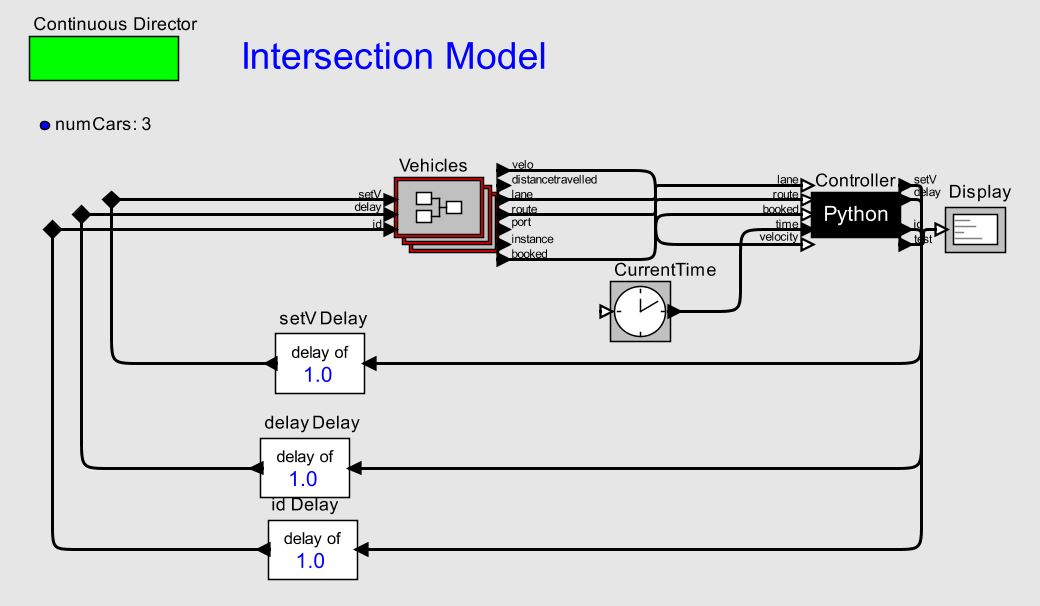
\includegraphics[width=0.9\linewidth]{diagram/ptolemy_system.jpg}
\end{frame}

\begin{frame}{Controller Algorithm}
\scriptsize
\begin{algorithmic}

\State {Initialize list of conflict zones and displacements along paths}
\For{each timestep $t$}
	\State $current \gets \text{all tokens received from Vehicle modal model}$
	\For{each $car$ in $current$}
		\If{$car$ needs reservation}
			\State {$v_\text{max} \gets$ maximum velocity
				$\in [ v_\text{current} \pm 10 ]$ that ensures safety}
			\If{$v_\text{max}$ exists}
				\State $v_\text{new} \gets v_\text{max}$
				\State $t_\text{delay} \gets 0$
			\Else
				\State $v_\text{new} \gets v_\text{current} + 10$
				\State $t_\text{delay} \gets$ end of latest reservation for all conflict zones
			\EndIf
			\State broadcast($v_\text{new}$, $t_\text{delay}$,
					$\text{id} \gets car\text{.id}$)
		\EndIf
	\EndFor
\EndFor

\end{algorithmic}
\end{frame}
